\chapter{ Terminierung des intrinsischen Delaunay-Refinements}
\label{kap:Terminierung}

Im Folgenden werden wir zeigen, dass der Algorithmus für eine Eingabe garantiert terminiert, für die alle Knoten $i$ einen Gesamtwinkel $\gesamtwinkel*\geq \frac{\pi}{3}$ haben und einen Winkel-Schwellenwert $\kleinsterWinkel* \leq \frac{\pi}{6}$. In der Ausgabe des Algorithmus soll für alle Innenwinkel der Triangulierung gelten, dass sie größer gleich dem gegebenen Winkel-Schwellenwert $\kleinsterWinkel*$ sind. Erst, wenn diese Bedingungen erreicht ist, terminiert der Algorithmus.


Da der Beweis mit  Längenrelationen arbeitet, führen wir Hilfsfunktionen ein, um Entfernungen besser zu beschreiben. 

\subsubsection{Hilfsfunktionen}
Die Hilfsfunktionen definieren verschiedene Längen, um später im Beweis mit ihnen arbeiten zu können.
\begin{definition}
Sei $M = (V,E,T)$ eine Delaunay-Triangulierung  einer geschlossenen StF-Oberfläche, sei $t \in T$ ein Dreieck aus $M$, sei $v,u \in V$ ein Knoten aus $M$ und sei $e_{(v,u)} \in V$ eine Kante aus $M$,  dann entspricht
\begin{itemize}
    \item $d(t)$ die Länge der kürzesten Seite von $t$
    \item $d(v)$ die Länge der kürzesten zu $v$ inzidenten Kante
    \item $d(v,u)$ die Länge der Kante  $e_{(v,u)}$
    \item $r(t)$ die Länge des Umkreisradius von $t$
    \item $N(v)$ einer Liste aller zu $v$ inzident Kanten
\end{itemize}


\end{definition}



Das folgende Lemma besagt, dass für einen Iterationsschritt die jeweils neu erzeugten Kanten adjazent zum neu eingefügten Knoten sind.


\begin{figure}[h!]
    \centering
    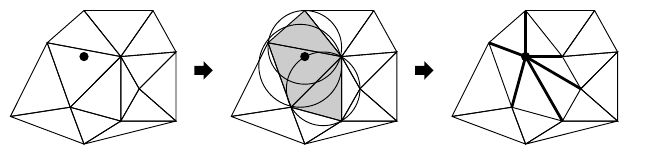
\includegraphics[width=5in]{images/adejazent.png}
    \caption{Illustration, dass alle neu erzeugten Kanten adjazent zum neu eingefügten Knoten sind~\cite{shewchuk:1997:delaunay}. }%\cite{shewchuk:1997:delaunay}}
    \label{fig:adejazent}
\end{figure}
 


\begin{lemma}
\label{le:adejazent}
Sei $M = (V,E,T)$ eine intrinsische Delaunay-Triangulierung  einer geschlossenen  StF-Oberfläche und sei $M^\prime = (V^\prime,E^\prime,T^\prime)$ die Delaunay-Triangulierung  $M$ nach dem Einfügen eines neuen Knotens $v$.\\
 

Wenn eine Kante $e \in E^\prime$ und $e \in N(v)$ ist und $e \in  N(v)$
dann folgt $e \not \in   E $.\\



\end{lemma}


\begin{proof}

 
Angenommen $e \not \in  N(v)$, dann ist zu zeigen, dass $e\in E $ gilt.\\

Nach~\cite[Definition 3]{Bobenko:2007:LaplaceBeltrami} ist eine Kante in einer Delaunay-Triangulierung  enthalten genau dann, wenn eine leere Kreisscheibe existiert, auf deren Rand nur ihre beiden Endknoten liegen.\\ 

    Wegen $V \subset V^\prime$  ist jede leere Kreisscheibe in $M^\prime$  auch in  $M$ enthalten. Per Annahme enthält $M$ auch beide Endknoten von $e$. Somit enthält $M$ auch $e$.     
\end{proof}


Dünne Dreiecke sind Dreiecke mit mindestens einem Innenwinkel $\leq \frac{\pi}{6}$.  
Das nächste Lemma zeigt, dass für ein dünnes Dreieck der Umkreisradius mindestens so lang ist wie seine kürzeste Kante.


\begin{lemma}
\label{le:dünnes_dreieck}
Sei $t$ ein Dreieck mit kleinstem Winkel $\alpha \leq \frac{\pi}{6}$.\\
Dann gilt: 
 
 \begin{align*}
     r(t) \geq d(t).
 \end{align*} 
 \end{lemma}

\begin{figure}[h]
    \centering
    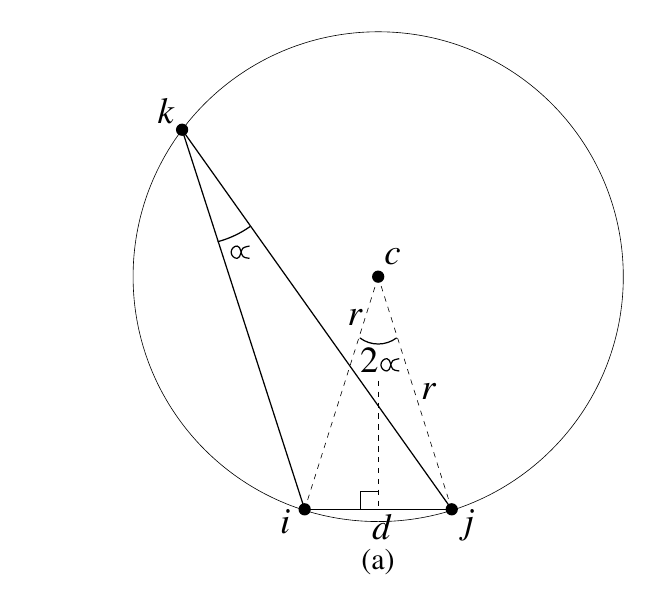
\includegraphics[width=3in]{images/Kreiswinkelsatz.png}
    \caption{Illustration des Kreiswinkelsatzes~\cite{shewchuk:1997:delaunay}}
    \label{fig:kreiswinkelsatz}
\end{figure}


\newpage
\begin{proof}
Mithilfe des Kreiswinkelsatzes (\ref{fig:kreiswinkelsatz}) gilt:
\begin{align*}
d(t) &= r(t)\cdot 2\cdot\sin(\alpha)  \\
\end{align*}
Aus der Annahme $\alpha \in [0,\frac{\pi}{6}] $ folgt:

\begin{align*}
    \sin(\alpha) \leq \frac{1}{2}.
\end{align*}

Einsetzen in obige Gleichung ergibt 

\begin{align*}
     d(t) &\leq r(t).\\
\end{align*}
\end{proof}

Das nächste Lemma zeigt, dass der größtmögliche Umkreisradius bereits in der Eingabe-Triangulierung enthalten ist und durch das Einfügen neuer Punkte nur leere Kreisscheiben erzeugt werden, deren Radius kleiner gleich dem größten Radius der Eingabe ist. 



Aufgrund der Delaunay-Eigenschaft gilt jedoch, dass in der Kreisscheibe (also nicht außerhalb und nicht auf dem Rand) keine Kugelpunkte liegen. Infolgedessen ist für eingebettete leere Kreisscheiben garantiert, dass alle beteiligten Flächen sich gemeinsam und eindeutig flach in der Ebene auffalten lassen. Somit können eingebettete leere Kreisscheiben, für sich genommen, wie in der Ebene behandelt werden. 



\begin{lemma}
\label{le:auffaltung}
Sei $M = (V,E,T)$ eine intrinsische Delaunay-Triangulierung  einer geschlossenen StF-Oberfläche. Sei $K$  die größte leere Kreisscheibe auf $M$ und sei $M^\prime = (V^\prime,E^\prime,T^\prime)$ die Delaunay-Triangulierung  $M$ nach dem Einfügen eines neuen Knotens $v$. 
Dann gilt für die größte leere Kreisscheibe $K^\prime$ in $M^\prime$,

\begin{align*}
    r(K) \geq r(K^\prime).\\
\end{align*}
\end{lemma}

\begin{proof}

Angenommen, durch das Einfügen von $v$ in $M$ entsteht eine neue leere Kreisscheibe $K^\prime$ mit 

\begin{align*}
    r(K^\prime) > r(K).
\end{align*}

Aus $V = V^\prime \setminus \{v\}$ und $K^\prime = \emph{}$ folgt $K^\prime \subset M$, da sie dann immer noch leer ist.\\ Das widerspricht der Annahme, dass $K$ die größte leere Kreisscheibe in $M$ ist.

\end{proof}






Bei der Triangulierung von geschlossenen StF-Oberfläche gibt es im Vergleich zu Triangulierungen in der euklidischen Ebene zusätzliche topologische Besonderheiten zu beachten. Da sie irreguläre Dreiecke zulassen, kann ein Knoten $v$ eine Kante \irregulaereKante zu sich selbst haben.    



Die minimale Länge von regulären Kanten wird dadurch festgelegt, dass Knoten nicht zu nahe beieinander eingefügt werden können. Dies gilt nicht für irreguläre Kanten.
Dabei ist es wichtig zu unterscheiden, ob sie sich um ein Loch, einen Bereich mit kurzem Umfang oder Kegelspitze wickelt. Bei einem Loch oder einem Bereich mit kurzem Umfang existiert ebenfalls ein festes Minimum, nämlich der minimale Umfang der StF-Oberfläche. Diese lässt sich berechnen~\cite{erickson:2005:generator}. Bei Kegelspitzen kann sich die Schleife  theoretisch unendlich klein zusammenziehen. Daher müssen wir diesen Fall gesondert betrachten.   




Da die Eingabetriangulierung im Allgemeinen regulär ist, können irreguläre Dreiecke erst durch das Wiederherstellen der Delaunay-Eigenschaft entstehen~\cite{Bobenko:2006:SIGGRAPH,Bobenko:2007:LaplaceBeltrami}. Wir betrachten den Fall einer Schleife um eine Kegelspitze und zeigen, dass die erzeugte irreguläre Kante größer gleich der regulären Kante ist.




 \begin{figure}[h]
    \centering
    


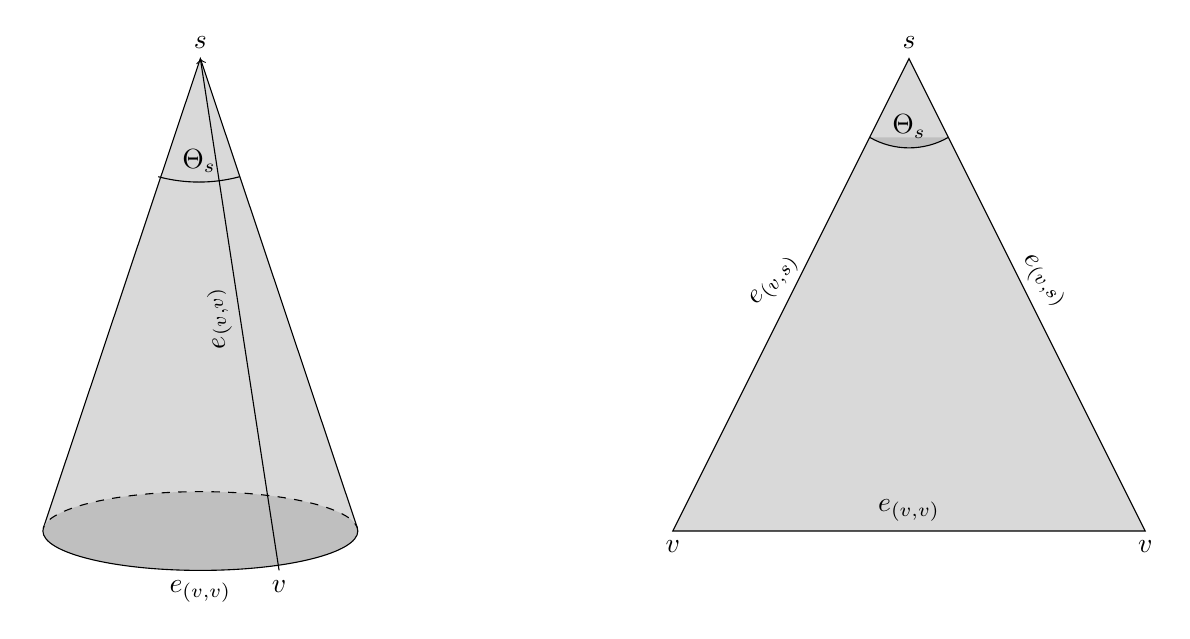
\begin{tikzpicture}

\usetikzlibrary{calc}
\newcommand{\radiusx}{2}
\newcommand{\radiusy}{.5}
\newcommand{\height}{6}

  \newcommand{\delayx}{6}

\coordinate (a) at (-{\radiusx*sqrt(1-(\radiusy/\height)*(\radiusy/\height))},{\radiusy*(\radiusy/\height)});

\coordinate (b) at ({\radiusx*sqrt(1-(\radiusy/\height)*(\radiusy/\height))},{\radiusy*(\radiusy/\height)});





\draw[fill=gray!30] (a)--(0,\height)--(b)--cycle;

\fill[gray!50] circle (\radiusx{} and \radiusy);

\begin{scope}
\clip ([xshift=-2mm]a) rectangle ($(b)+(1mm,-2*\radiusy)$);
\draw circle (\radiusx{} and \radiusy);
\end{scope}

\begin{scope}
\clip ([xshift=-2mm]a) rectangle ($(b)+(1mm,2*\radiusy)$);
\draw[dashed] circle (\radiusx{} and \radiusy);
\end{scope}

%\draw[dashed] (0,\height)|-(\radiusx,0) node[right, pos=.25]{$h$} node[above,pos=.75]{$r$};
%\draw (0,.15)-|(.15,0);


\draw  ( 0,\height) coordinate (a)  (\radiusx,0) coordinate (b) (-1* \radiusx ,0) coordinate (c); 

% \pic[draw=orange,<->,angle radius=\radiusx * 20,fill=teal!30]{angle=c--a--b};
\draw  (0+0.5,\height-1.5) arc (-75:-105:2) node[above,midway]{$\Theta_{s}$};


\draw[->](\radiusx/2,-\radiusy)--node[above,rotate=100] {$e_{(v,v)}$} (0,\height);
\coordinate[label=below:$v$] (d)  at (\radiusx/2,-\radiusy);
\coordinate[label=below:$e_{(v,v)}$] (d)  at (0,-\radiusy);
\coordinate[label=above:$s$] (c) at (0,\height);


\draw[fill=gray!30]   (0+\delayx,0) coordinate[label=below:$v$] (a) -- node[above,rotate=50] {$e_{(v,s)}$} 
        (3+\delayx,6) coordinate[label=above:$s$] (b) -- node[above,rotate=-50] {$e_{(v,s)}$}
        (6+\delayx,0) coordinate[label=below:$v$] (c) --node[above] {$e_{(v,v)}$}  cycle;
        
    \draw[fill=gray!50]  ({3+\delayx+.5},{6-1}) arc (-60:-120:1) node[above,midway]{$\Theta_{s}$};
    




\end{tikzpicture}


    \caption{Illustration der Auffaltung eines irregulären Dreiecks in der euklidischen Ebene.}%\cite{shewchuk:1997:delaunay}}
    \label{fig.irreglaere}
\end{figure}

\begin{lemma}
\label{le:irregulär_entfernung}
Sei $M = (V,E,T)$ eine intrinsische Delaunay-Triangulierung  einer geschlossenen  StF-Oberfläche und  $t \in T$ ein irreguläres Dreieck aus $M$. 


Seien $v,s \in V$ die Knoten von t, \irregulaereKante die irreguläre Kante und Kegelwinkel \gesamtwinkel[s] von s gilt $\gesamtwinkel*[s] \in [\frac{\pi}{3}, \pi].$


Dann folgt:
\begin{align*}
    d(\irregulaereKante*) \geq d(\regulaereKante*).\\
\end{align*}  
\end{lemma}

\begin{proof}

Aus dem Kosinussatz folgt 
\begin{align*}
    d(\irregulaereKante*^2) &=  d(e_{(s,v)})^2 + d(e_{(v,s)})^2-2 \cdot d(e_{(s,v)})  \cdot d(e_{(v,s)}) \cdot \cos(\gesamtwinkel*[s]). \\
\end{align*}

Da $d(e_{(s,v)}) = d(e_{(v,s)})$ gilt, erhalten wir durch Umformung

\begin{align*}
d(\irregulaereKante*)&= \sqrt{2 (1-\cos(\gesamtwinkel*[s]))}\cdot d(\regulaereKante*).\\
\end{align*}

Wegen $\gesamtwinkel*[s] \in  [\frac{\pi}{3}, \pi]$, also $-1 \leq \cos(\gesamtwinkel*[s]) \leq \frac{1}{2}$  folgt

\begin{align*}
     \sqrt{2 (1-\cos(\gesamtwinkel*[s]))} \geq \sqrt{2 (1-\frac{1}{2})} \geq 1\\
\end{align*}

und damit $\irregulaereKante* \geq \regulaereKante* $. 


\end{proof}



Das folgende Lemma zeigt, dass durch den Algorithmus erzeugte reguläre Kanten nicht kleiner als der entsprechende Umkreisradius $r(t_{bad})$ des dünnen Dreiecks $t_{bad}$ sein können, aus dem sie erzeugt wurden.

\newpage
\begin{lemma}
\label{le:regulär_entfernung}
Sei $M = (V,E,T)$ eine Delaunay-Triangulierung  einer geschlossenen StF-Oberfläche, sei $t \in T$ ein Dreieck aus $M$, sei $v$ der Umkreismittelpunkt von $t$.   \\

 



Nach dem Einfügen von $v$ in $M$ und der Wiederherstellung der Delaunay-Eigenschaft gilt für jede neu erzeugte reguläre Kante $e$, dass sie adjazent zu $v$ ist, und dass 
\begin{align*}
    d(e) \geq r(t) 
\end{align*} gilt.

\end{lemma}
 \begin{figure}[h]
    \centering
    \includegraphics[width=3in]{images/regulär_entfernung.png}
    \caption{Illustration, dass durch die Delaunay-Eigenschaft gewährleistet wird, dass neu eingefügte Knoten nicht zu nahe an bestehen Knoten liegen    \cite{SHEWCHUK:2002:chuws}.}
    \label{fig:regulär_entfernung}
\end{figure}

\begin{proof}
Da $M$ die Delaunay-Eigenschaft besitzt, gilt für alle Dreiecke $t\in T$ die Delaunay-Eigenschaft, die besagt, dass im Umkreis von $t$ keine Knoten liegen, die nicht zu $t$ gehören. Nach dem Einfügen von $v$ in $M$ und dem Wiederherstellen der Delaunay-Eigenschaft gilt also für alle neu hinzugefügten regulären Kanten, dass sie inzident zu $v$ (\ref{le:adejazent}) und somit mindestens $r(t)$ lang sind.
\end{proof}

\newpage
Der folgende Beweis vereint nun die in den Lemmata aufgestellten Längenrelationen und zeigt, dass der Algorithmus nur Kanten erzeugen kann, die eine, durch die Eingabe bestimmte, Mindestlänge haben.

\begin{lemma}
\label{lem:Obergrenze}
Sei $M = (V,E,T)$ eine Delaunay-Triangulierung   einer geschlossenen StF-Oberfläche, sei $d_{min}$ die kürzeste Distanz zwischen zwei Knoten von $M$, sei $g_{min}$ der kürzeste Umfang von $M$ und sei $K_{max}$ die größte leere Kreisscheibe von $M$.

Angenommen, $M$ hat keine Kegelspitze $s$ mit einem Gesamtwinkel $\gesamtwinkel*[s] \leq \frac{\pi}{3}$. 

dann  existiert ein 
\begin{align*}
    \kappa^* = \frac{\min(d_{min}, g_{min} )}{r(K_{max)}}
\end{align*}
mit 
\begin{align*}
 \kappa^* \leq \kappa   
\end{align*}
für alle Dreiecke aus $M$.




\end{lemma}



\begin{proof}

Laut Lemma~\ref{le:auffaltung} kann der Algorithmus keine Umkreisradien größer $r(k_{max})$ erzeugen.

Nehmen wir an, dass der Algorithmus \textit{intrinsisches Delaunay-Refinement} eine Kante, die kürzer als $\min(d_{min}, g_{min} )$ ist, einfügt. Sei~\regulaereKante[(v,u)] die erste Kante dieser Art. Nach Lemma~\ref{le:adejazent} ist \regulaereKante[(v,u)] inzident zum zuletzt eingefügten Knoten. Sei dieser $v$ und $t_{bad}$ das zugehörige dünne Dreieck. \\

Da vor dem Einfügen von $v$ keine Kante kürzer als $\min(d_{min}, g_{min} )$ existiert hat, gilt  
\begin{align*}
    d(t_{bad}) \geq d_{min}.\\
\end{align*} 

Gemäß Lemma~\ref{le:irregulär_entfernung} und~\ref{le:regulär_entfernung} gilt, wenn \regulaereKante[(v,u)] eine reguläre Kante oder eine irreguläre Kante um eine Kegelspitze ist, die Abschätzung

\begin{align*}
    d(\regulaereKante*[(v,u)]) \geq r(t_{bad}).\\
\end{align*} 


Da $t_{bad}$ dünn ist, gilt nach Lemma~\ref{le:dünnes_dreieck} 
\begin{align*}
    r(t_{bad}) \geq d(t_{bad}).
\end{align*}


 Daraus folgt  
 \begin{align*}
     d(\regulaereKante*[(v,u)]) \geq d_{min}.
 \end{align*}

Weiterhin gilt, wenn \regulaereKante[(v,u)] eine Schleife um einen Bereich mit kurzem Umfang oder ein Loch ist, nach Definition

\begin{align*}
     d(\regulaereKante*[(v,u)]) \geq g_{min}.
 \end{align*}



Das steht jedoch im Widerspruch zu der Annahme, dass \regulaereKante[(v,u)] kürzer ist als $\min(d_{min}, g_{min} )$. Es folgt also, dass keine eingefügte Kante kürzer ist als $\min(d_{min}, g_{min} )$. Somit kann der Algorithmus keine Dreiecke erzeugen, für die gilt \\
 \begin{align*}
    \kappa^* = \frac{ \min(d_{min}, g_{min} )}{r(k_{max})} \leq \kappa.
 \end{align*}

\end{proof}

In Lemma~\ref{lem:Obergrenze} haben wir gezeigt, dass der Algorithmus nur Dreiecke erzeugt mit $\kappa \geq \kappa* $.

Nun wollen wir zeigen, dass das intrinsische Delaunay-Refinement aufgrund der begrenzten Fläche terminiert. Da die Fläche der Eingabetriangulierung endlich ist, der Algorithmus in jeder Iteration neue Dreiecke erzeugt und diese Dreiecke wiederum eine Mindestfläche $A_{min}$ haben, folgt, dass der Algorithmus terminieren muss, sobald er die zur Verfügung stehende Gesamtfläche nicht mehr weiter aufteilen kann.\\  



\begin{theorem}
Sei $M = (V,E,T)$ eine Triangulierung einer geschlossenen StF-Oberfläche.
Angenommen, $M$ hat keine Kegelspitze $s$ mit einem Gesamtwinkel $\gesamtwinkel*[s] \leq \frac{\pi}{3}$ und sei  $\kleinsterWinkel* \leq \frac{\pi}{6}$ ein Winkel-Schwellenwert. 


Das intrinsische Delaunay-Refinement mit $M$ und \kleinsterWinkel als Eingabe terminiert.
\end{theorem}



\begin{proof}
das Lemma~\ref{lem:Obergrenze} zeigt, dass es keine Kante kürzer ist als  \begin{align*}
    D = \min(d_{min},g_{min})
\end{align*}

und eine Untergrenze \begin{align*}
    \kappa^* \leq \frac{\min(d_{min},g_{min})}{r(k_{max})}
\end{align*}

von $\kappa$ existiert.

Aus dem Kreiswinkelsatz folgt, es existiert ebenfalls eine Winkeluntergrenze 

\begin{align*}
    A = \sin(\frac{\kappa^*}{2})
\end{align*}
für jedes Dreieck.\\
Aus dem Sinussatz folgt, dass jedes Dreieck eine Mindestfläche von \begin{align*}
    \frac{1}{2} \cdot \sin(A)D^2 
\end{align*}
hat.\\

Insgesamt ist die Fläche der Eingabetriangulierung begrenzt und jedes Dreieck hat eine Mindestfläche. Der Algorithmus erzeugt in jedem Schritt neue Dreiecke und da der Algorithmus nur Dreiecke mit endlich kleine Flächen erzeugen kann, muss er schließlich terminieren.
\end{proof}








